\documentclass[border=5pt]{standalone}
\usepackage{tikz}

\begin{document}
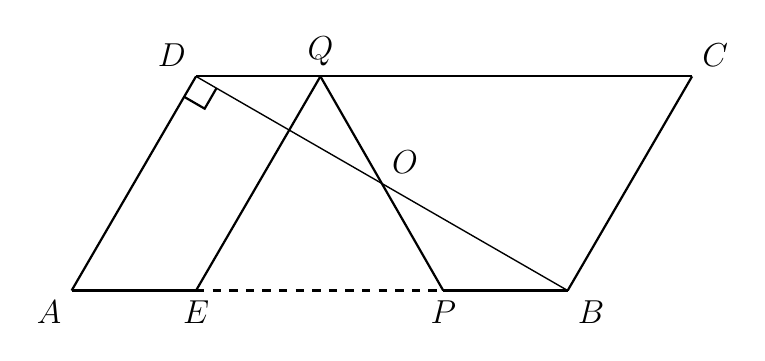
\begin{tikzpicture}[thick,
  every node/.style={font=\large}]

  % 坐标
  \coordinate (A) at (1.32,0);
  \coordinate (B) at (7.62,0);
  \coordinate (C) at (9.20,2.72);
  \coordinate (D) at (2.90,2.72);
  \coordinate (E) at (2.90,0);
  \coordinate (P) at (6.04,0);
  \coordinate (Q) at (4.48,2.72);
  \coordinate (O) at (5.26,1.36);

  % 平行四边形边：AE 与 PB 实线，EP 虚线
  \draw (A) -- (E);
  \draw[dashed] (E) -- (P);
  \draw (P) -- (B);
  \draw (B) -- (C);
  \draw (C) -- (D);
  \draw (D) -- (A);

  % 线段 QE、QP
  \draw (Q) -- (E);
  \draw (Q) -- (P);

  % 对角线 DB（细线）
  \draw[line width=0.5pt] (D) -- (B);

  % 直角标记（∠ADB）
  \draw (2.75,2.46) -- (3.01,2.31) -- (3.16,2.57);

  % 标签
  \node[below left]  at (A) {$A$};
  \node[below]       at (E) {$E$};
  \node[below]       at (P) {$P$};
  \node[below right] at (B) {$B$};
  \node[above right] at (C) {$C$};
  \node[above left]  at (D) {$D$};
  \node[above]       at (Q) {$Q$};
  \node[above right] at (O) {$O$};

\end{tikzpicture}
\end{document}
